%%%%%%%%%%%%%%%%%%%%%%%%%%% COORDINATESYSTEMS
% COORDSYS (ORIGOCOORDINATENAME, WIDTH, HEIGHT)
% Draws a Coordinatesystem around ORIGOCOORDINATENAME with a width of WIDTH and a height of HEIGHT, 
% names the beginning and end of axes, southwest corner, northwest corner, 
\newcommand{\OneQuadrantCoordSys}[3]{
\coordinate (XY#1) at ([xshift=#2 cm, yshift=#3 cm]#1);
%\coordinate (-XY#1) at ([xshift=-#2 cm, yshift=-#3 cm]#1);
%\coordinate (-X#1) at ([xshift=-#2 cm]#1);
\coordinate (X#1) at ([xshift=#2 cm]#1);
\coordinate (Y#1) at ([yshift=#3 cm]#1);
%\coordinate (-Y#1) at ([yshift=-#3 cm]#1);
%\draw [help lines, step=.5cm] (#1) grid (XY#1);
\draw[->, name path=XAxis#1] (#1)--(X#1);
\draw[->, name path=YAxis#1] (#1)--(Y#1);
}

% \DistanceLabel{SS}{AS}{-45}{1}{pos=.5}{1}
\newcommand{\DistanceLabel}[6]{
\coordinate(#1horgony) at ([shift=(#3:#4)] #1);
\coordinate(#2horgony) at ([shift=(#3:#4)] #2);
\draw[thin, red, <->] (#1horgony)--(#2horgony) node[#5, scale=.7]{#6};
\draw[opacity=.4, black] (#1)--(#1horgony);
\draw[opacity=.4, black] (#2)--(#2horgony);
}

%Lorentz(OriginalOriginCoord, ResultingOriginCoord, SpeedNum, PointCoord, Label)
% 
\newcommand{\Lorentz}[5]{
\path (#1); \pgfgetlastxy{\XCoord}{\YCoord}; % Extracting coordinates of the Origin
\pgfmathsetmacro{\XOrigin}{\XCoord} % Saving X coordinate
\pgfmathsetmacro{\YOrigin}{\YCoord} % Saving Y coordinate
\path (#4); \pgfgetlastxy{\XCoord}{\YCoord}; % Extracting coordinates of the Point
\pgfmathsetmacro{\XEvent}{\XCoord} % Saving X coordinate
\pgfmathsetmacro{\YEvent}{\YCoord} % Saving Y coordinate
\pgfmathsetmacro{\XEventWRTOrigin}{\XEvent-\XOrigin} % Relativizing to the origin
\pgfmathsetmacro{\YEventWRTOrigin}{\YEvent-\YOrigin} % Relativizing to the origin
\pgfmathparse{XLorentz(#3,\XEventWRTOrigin,\YEventWRTOrigin)} % transforming x
\pgfmathsetmacro{\XEventTr}{\pgfmathresult} % save the result of x
\pgfmathparse{YLorentz(#3,\XEventWRTOrigin,\YEventWRTOrigin)} % transforming y
\pgfmathsetmacro{\YEventTr}{\pgfmathresult} % save the result of y
\node[inner sep=0](#5) at (
[xshift=\XEventTr pt,
 yshift=\YEventTr pt] #2){};
}

\usetikzlibrary{calc}
\usetikzlibrary{intersections}
\newdimen\XCoord
\newdimen\YCoord

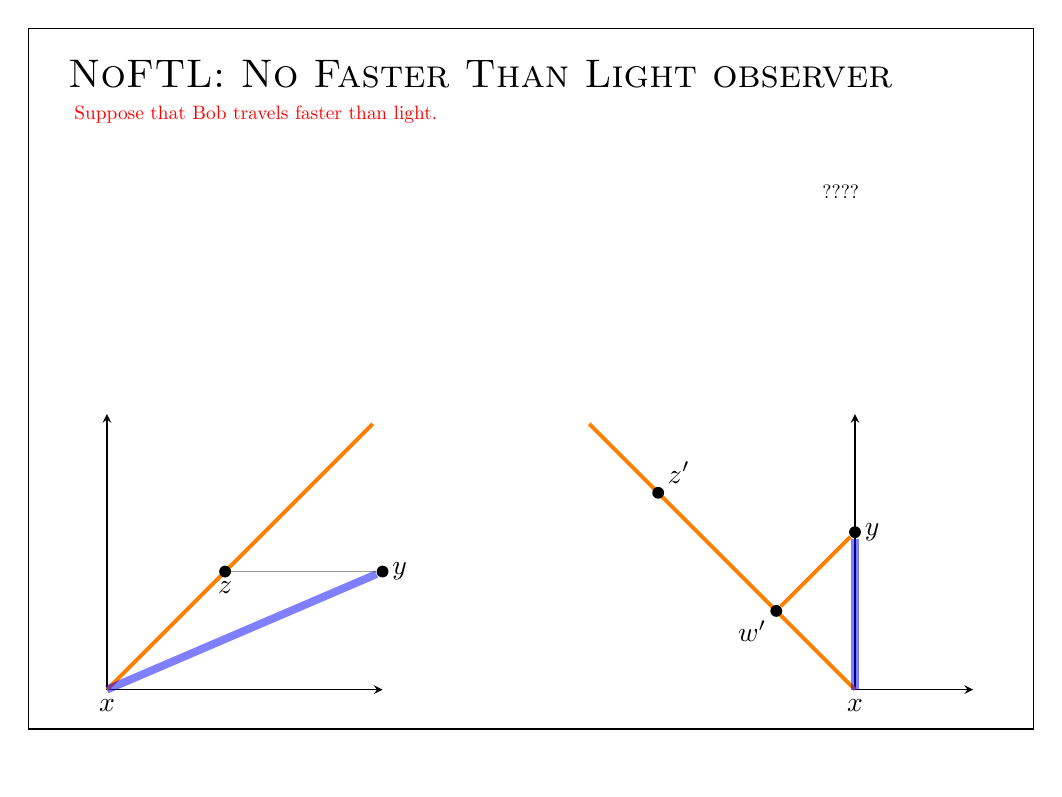
\begin{tikzpicture}[>=stealth, scale=1,
world/.style={inner sep=0, minimum size=.15cm, fill=black, circle},
worldline/.style={line width=1mm, rounded corners=1pt, opacity=.5},
axis/.style={->},
light/.style={orange, line width=.5mm},
]
\pgfmathdeclarefunction{XLorentz}{3}{\pgfmathparse{(#2 - #1*#3)/(sqrt(1-#1^2))}} % speed, spacecoord, timecoord
\pgfmathdeclarefunction{YLorentz}{3}{\pgfmathparse{(#3 - #1*#2)/(sqrt(1-#1^2))}} % speed, spacecoord, timecoord
\pgfmathsetmacro{\ThirdAxisAngle}{-135}
\pgfmathsetmacro{\ThirdAxisUnit}{.7}

%%%%%%%%%%%%%%%%%%%%%%%% DIA KEZDETE %%%%%%%%%%%%%%%%%%%%%%%%%%%

\node[anchor=north west, inner sep=0] at (0.5,8.5) {\textsc{\Large NoFTL: No Faster Than Light observer}}; %%%%%%% TITLE
%\node[anchor=north west, inner sep=0] at (0.5,8) {\textsc{\normalsize Role of Light}}; %%%%%%% SUBTITLE
\draw%[white]  %%%%%%%%%%%% SIZE OF THE SLIDE
      (0,0) rectangle (12.77,8.9);
%%%%%%%%% TEXT %%%%%%%%%%%%%
\node[anchor=north west, fill=white, fill opacity=1, text opacity=1,scale=.7] at (0.5,8) 
{\begin{minipage}{9cm}
\textcolor{red}{Suppose that Bob travels faster than light.}
\end{minipage}
};
%%%%%%%%%%%%%%%%%%%%%%%% KOORDINÁTARENDSZEREK %%%%%%%%%%%%%%%%%%%%%%%%%%%
\coordinate(O1) at (1,0.5);
  \OneQuadrantCoordSys{O1}{3.5}{3.5}{3}
\coordinate(O2) at (10.5,0.5) {} {} {};
  \OneQuadrantCoordSys{O2}{1.5}{3.5}{3}

%%%%%%%%%%
%% SETTINGS %%
%%%%%%%%%%

\coordinate (AliceStart) at (O1);
\coordinate (AliceEnd) at (1,4);
\coordinate (BobStart) at (O1); % Fontos hogy átmenjen az Origón, különben rossz a lorentz transzformáció!!
\coordinate (BobEnd) at (0.5,4) {};

%%%%%%%%%%% Ezt lehetne macronak, speedszámítócuccnak
\path (BobStart); \pgfgetlastxy{\XCoord}{\YCoord}; % Extracting coordinates of the Origin
\pgfmathsetmacro{\XFirst}{\XCoord} % Saving X coordinate
\pgfmathsetmacro{\YFirst}{\YCoord} % Saving Y coordinate
\path (BobEnd); \pgfgetlastxy{\XCoord}{\YCoord}; % Extracting coordinates of the Point
\pgfmathsetmacro{\XSecond}{\XCoord} % Saving X coordinate
\pgfmathsetmacro{\YSecond}{\YCoord} % Saving Y coordinate
\pgfmathsetmacro{\SpeedBob}{(\XFirst-\XSecond)/(\YFirst-\YSecond)} % Relativizing to the origin
%%%%%%%%%%%%%%%%%%%%%%%%%%%%%%%%%%%

\Lorentz{O1}{O1}{0}{BobStart}{BS}
\Lorentz{O1}{O1}{0}{BobEnd}{BE}

\Lorentz{O1}{O2}{\SpeedBob}{AliceStart}{AS'}


\node[anchor=north west, scale=.7] at (10,7) {
\begin{minipage}{2cm}
????\end{minipage}};


\node[world] (y) at (4.5,2) {};
\node (v1) at (4.5,4) {};

\draw[light, name path=LIGHT]  (O1) -- (v1);
\draw[worldline, blue]  (O1) -- (y);
\node(v1') at (7,4) {};
\draw[light, name path=LIGHT']  (O2) -- (v1');
\node[world] (y') at (10.5,2.5) {};
\draw[worldline, blue]  (O2) edge (y');
\node[anchor=north] at (O1){$x$};
\node[anchor=west] at (y){$y$};
\node[anchor=north] at (O2){$x$};
\node[anchor=west] at (y'){$y$};



%\pause %%%%%%%%%%%%%%% PAUSE

\coordinate(refy) at ([xshift=-3cm]y);
\path[name path=horizonv2] (refy)--(y);
\node[world, name intersections={of=horizonv2 and LIGHT, by=z}]at (z){};
\draw[opacity=.4] (z)--(y);
\node[anchor=north] at (z){$z$};

%\pause %%%%%%%%%%%%%%% PAUSE

\node[world](z') at (8,3) {};
\node[anchor=south west] at (z') {$z'$};

%\pause %%%%%%%%%%%%%%% PAUSE

\coordinate(refy') at ([xshift=-3cm, yshift=-3cm]y');
\path[name path=lightline] (refy')--(y');
\node[world, name intersections={of=lightline and LIGHT', by=w'}](w'node)at (w'){};
\draw[light] (w'node)--(y');
\node[anchor=north east] at (w'){$w'$};



\end{tikzpicture}